\documentclass[onecolumn, draftclsnofoot,10pt, compsoc]{IEEEtran}
\usepackage{graphicx}
\usepackage{caption}
\usepackage{amsmath}
\usepackage{amssymb}
\usepackage{url}
\usepackage{setspace}

\usepackage{geometry}
\geometry{textheight=9.5in, textwidth=7in}

% 1. Fill in these details
\def \CapstoneTeamName{		Gesture Recognition}
\def \CapstoneTeamNumber{		33}
\def \GroupMemberOne{			Jonathan Hull}
\def \GroupMemberTwo{			Nicholas Davies}
\def \GroupMemberThree{			Shane Clancy}
\def \GroupMemberFour{          Shihao Song}
\def \GroupMemberFive{          Ulises Zaragoza}
\def \GroupMemberSix{           Zhidong Zhang}
\def \CapstoneProjectName{		Gesture Recognition using new Intel Real Sense light coded Camera}
\def \CapstoneSponsorCompany{ Intel}
\def \CapstoneSponsorPersonOne{		Eduardo X. Alban}
\def \CapstoneSponsorPersonTwo{        Satoshi Suzuki}
\def \CapstoneSponsorPersonThree{        Po-Cheng Chen}

% 2. Uncomment the appropriate line below so that the document type works
\def \DocType{	%Problem Statement
				%Requirements Document
				%Technology Review
				Design Document
				%Progress Report
				}
			
\newcommand{\NameSigPair}[1]{\par
\makebox[2.75in][r]{#1} \hfil 	\makebox[3.25in]{\makebox[2.25in]{\hrulefill} \hfill		\makebox[.75in]{\hrulefill}}
\par\vspace{-12pt} \textit{\tiny\noindent
\makebox[2.75in]{} \hfil		\makebox[3.25in]{\makebox[2.25in][r]{Signature} \hfill	\makebox[.75in][r]{Date}}}}
% 3. If the document is not to be signed, uncomment the RENEWcommand below
%\renewcommand{\NameSigPair}[1]{#1}

%%%%%%%%%%%%%%%%%%%%%%%%%%%%%%%%%%%%%%%
\begin{document}
\begin{titlepage}
    \pagenumbering{gobble}
    \begin{singlespace}
    	%\includegraphics[height=4cm]{coe_v_spot1}
        \hfill 
        % 4. If you have a logo, use this includegraphics command to put it on the coversheet.
        %\includegraphics[height=4cm]{CompanyLogo}   
        \par\vspace{.2in}
        \centering
        \scshape{
            \huge CS Capstone \DocType \par
            {\large\today}\par
            \vspace{.5in}
            \textbf{\Huge\CapstoneProjectName}\par
            \vfill
            {\large Prepared for}\par
            \Huge \CapstoneSponsorCompany\par
            \vspace{5pt}
            {\Large\NameSigPair{\CapstoneSponsorPersonOne}\par}
            {\Large\NameSigPair{\CapstoneSponsorPersonTwo}\par}
            {\Large\NameSigPair{\CapstoneSponsorPersonThree}\par}
            {\large Prepared by }\par
            Group\CapstoneTeamNumber\par
            % 5. comment out the line below this one if you do not wish to name your team
            \CapstoneTeamName\par 
            \vspace{5pt}
            {\Large
                \NameSigPair{\GroupMemberOne}\par
                \NameSigPair{\GroupMemberTwo}\par
                \NameSigPair{\GroupMemberThree}\par
                \NameSigPair{\GroupMemberFour}\par
                \NameSigPair{\GroupMemberFive}\par
                \NameSigPair{\GroupMemberSix}\par
            }
            \vspace{20pt}
        }
        \begin{abstract}
        Our group has broken up our project into three key components: the User Interface, the Software, and Machine Learning project portions. These components will work together following the Dependency Inversion Principle, and can developed independently from one another. Once these separate components are fully developed they will be integrated and reliant upon one another, with a flow of data running through each of the segments and exchange points occurring during Software project portions. With this pipeline defined, our group has identified the major functionalities needed to be accomplished within each component's domain. This document highlights the required tasks needed within each key project component.
        	
        \end{abstract}     
    \end{singlespace}
\end{titlepage}
\newpage
\pagenumbering{arabic}
\tableofcontents
% 7. uncomment this (if applicable). Consider adding a page break.
%\listoffigures
%\listoftables
\clearpage

% 8. now you write!

\section{Introduction}
\subsection{Purpose}
Our group is expected to train a machine learning (ML) classification model, with the task of having the model accurately identify human gestures from the Intel RealSense camera input feed. We are also expected to build a program with a GUI interface to present the text representation of classified gestures. Furthermore, the motivation behind this project includes the desire to create a cost effective and accessible system that aids people in communicating in more effective ways. Our end goal is to be able to identify American Sign Language gestures using our ML model wrapped in the GUI application. This opens up the possibility of aiding individuals with difficulty using speech as a primary communication medium.
\subsection{Scope}
The system scope of our project has an end goal of having a ML model be able to classify sign-language gestures, and present this classification via a text message to the user through the housing GUI application. Our project will take on a small initial scope, as we seek to first build and train a foundation ML model that can perform basic gesture recognition tasks such as identifying a hand waving. Once this has been established, we will work to fine-tune the model and prepare it to handle our end-goal task of American Sign-Language recognition in real-time from video camera feeds.

\subsection{Glossary}
\begin{itemize}
    \item UI - User Interface
    \item SW - Software
    \item ML - Machine Learning
    \item GUI - Graphical User Interface
    \item CNN - Convolutional Neural Network
\end{itemize}

\subsection{Intended Audience}
Our client and direct audience for this document is primarily the Intel stakeholders identified on the cover page, and associated group members. For the users of this project, the intended audience would be those in the deaf community or any in need of a gesture recognition software, bundled with the RealSense Camera. The end goal, as identified by stakeholders, is to create a software tailored to those who may require aid with speech communication. We will keep this specific audience in mind as we begin implementation.

\subsection{Design Timeline}
The figure below displays the timeline for our group's separate key project components, the User Interface (UI), Soft-Ware Interface (SW) and Machine Learning (ML) project portions. As noted from the Gantt Chart timeline below, the key milestones for the UI team include two separate goals of producing an initial basic UI that can perform a simple capture, followed by an advanced UI version that will ultimately be our final interface production model. The SW team has four major goals of creating a Data collection tool and implementing a storage method, performing pre-processing data manipulations, and implementing UI \& SW interfacing capabilities. The ML team has four major goals which include creating a baseline CNN architecture, preparing the algorithm to receive camera input, train for basic gesture recognition, and then training for advanced gesture recognition. These tasks are planned such that each team may work semi-independently from one another, until the interfacing connections by the SW team must be implemented.
 \begin{figure}[ht]
    \centering
    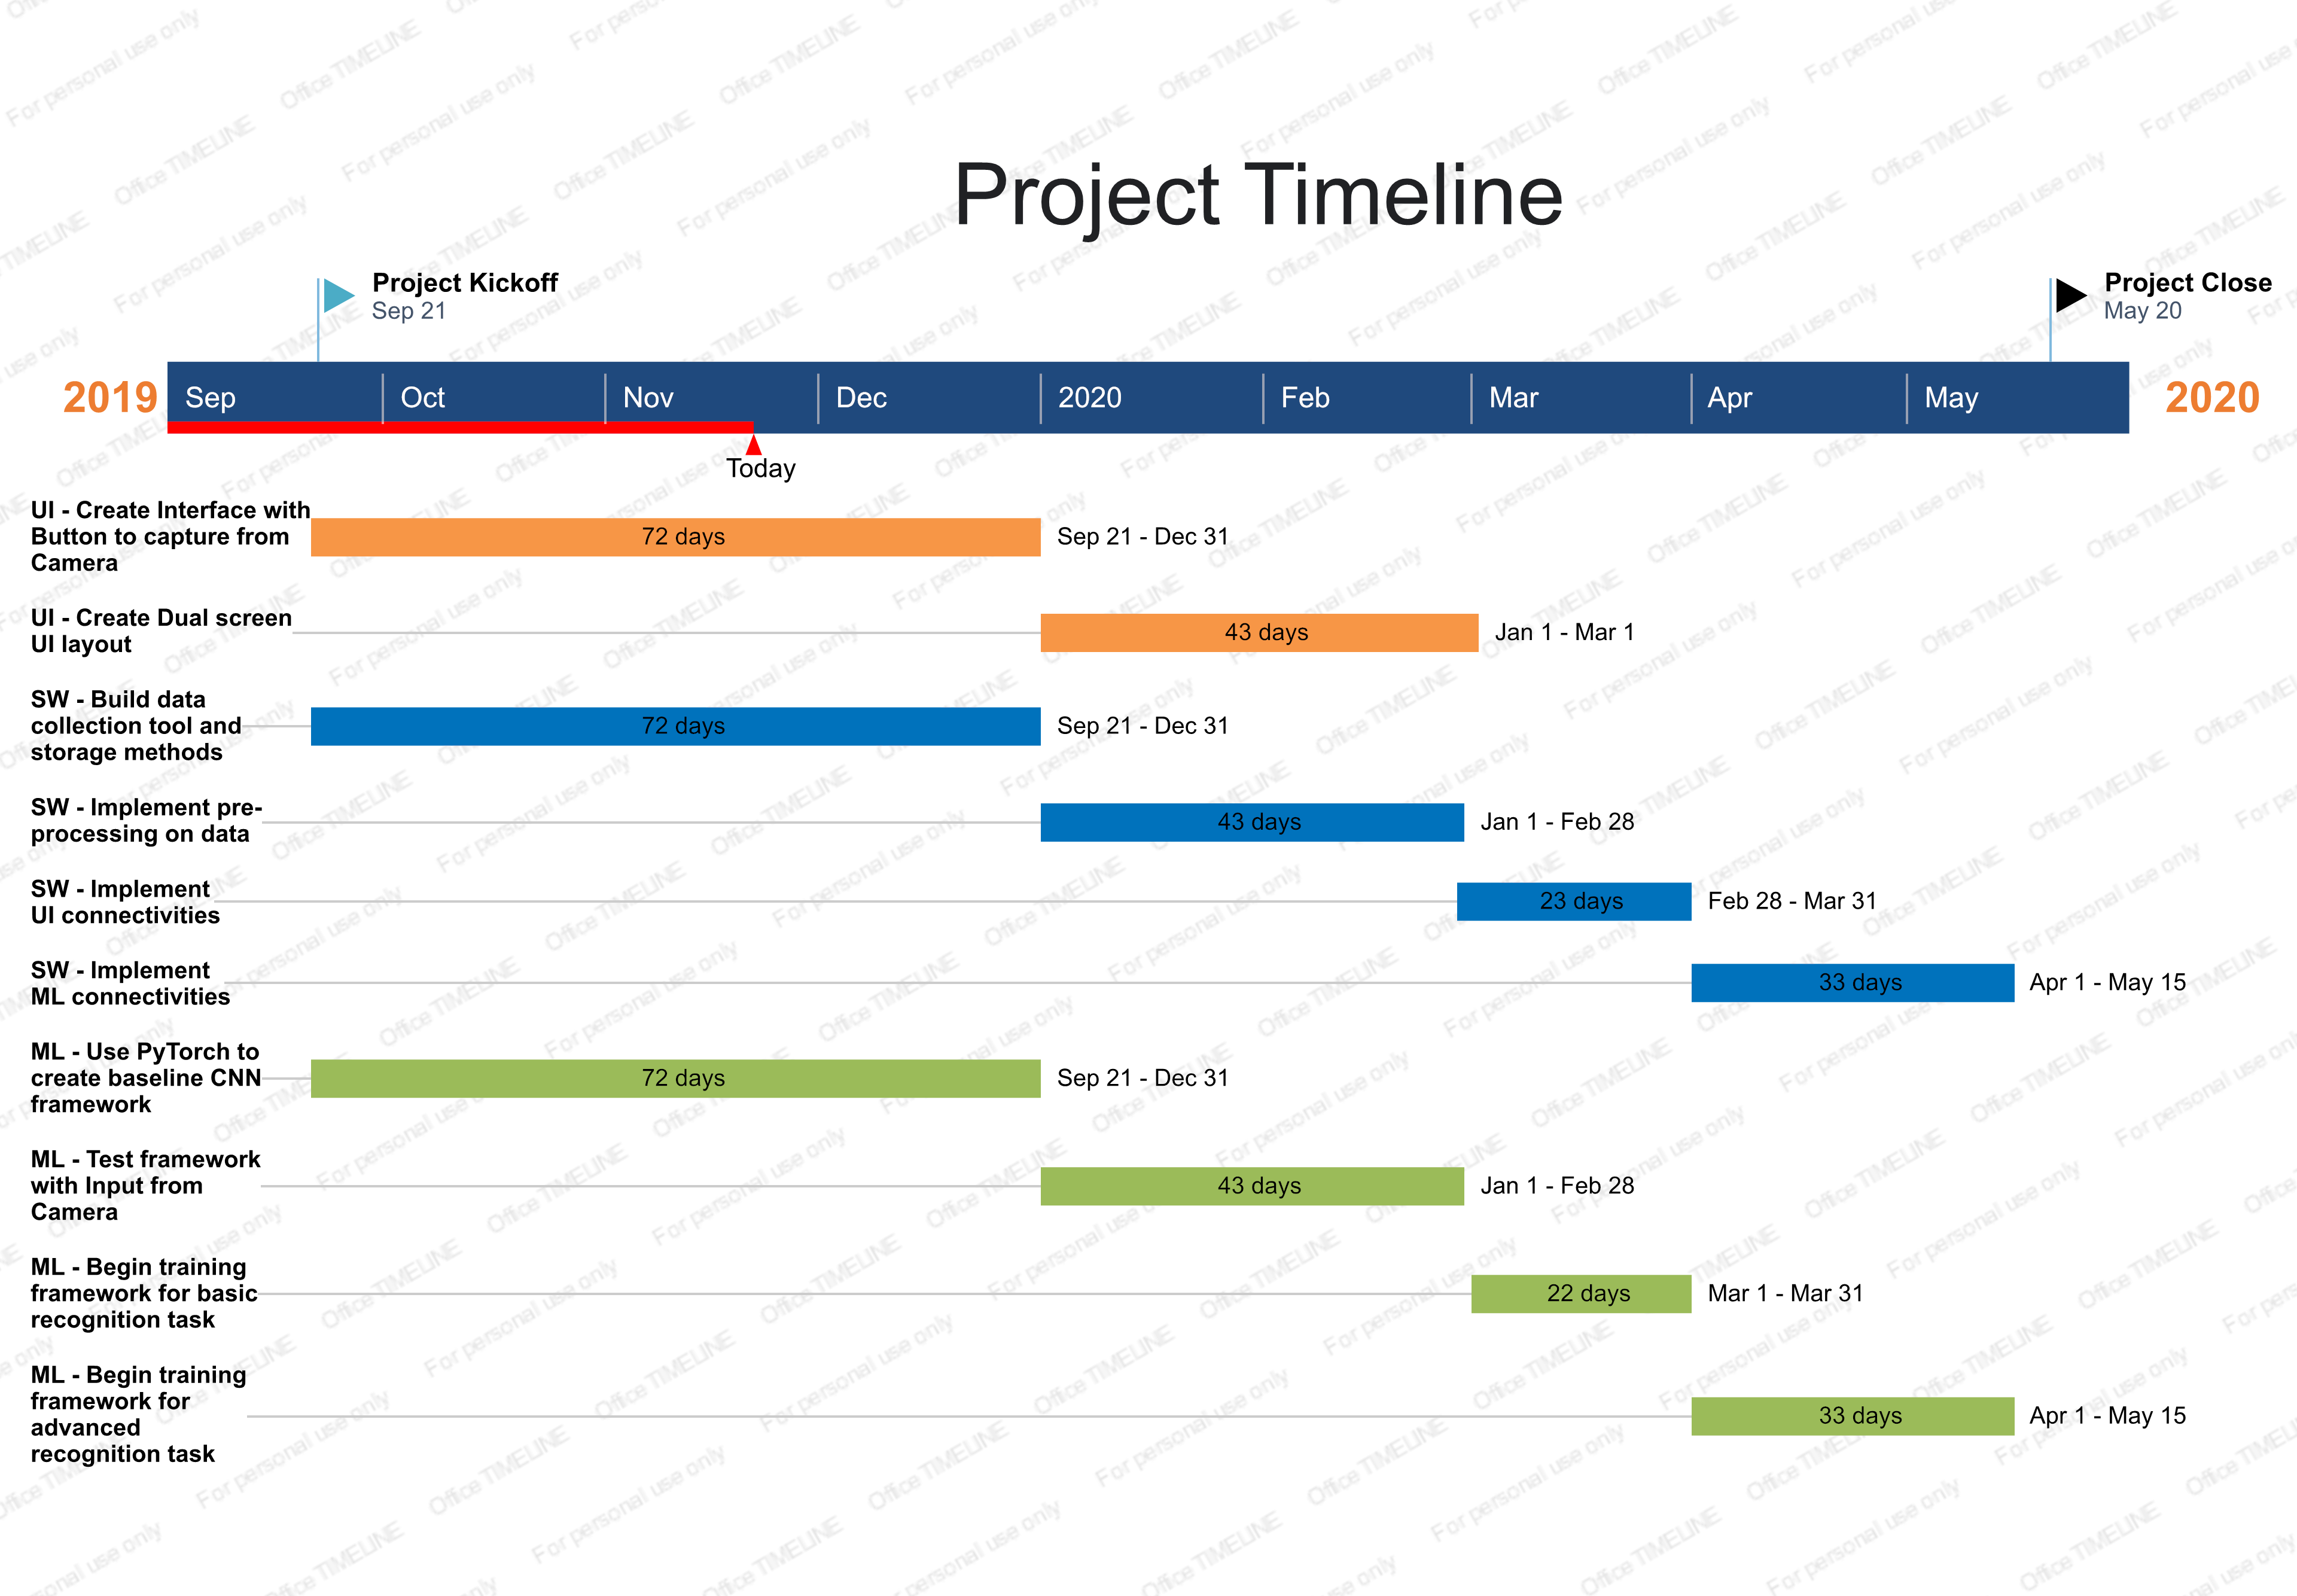
\includegraphics[width=1.0\textwidth]{GanttChart.png}
    \caption{Project Timeline}
    \label{fig:Figure 1}
\end{figure}


\section{Design}
\subsection{Viewpoint : User Interface Design}
\subsubsection{Introduction}
A major component of this project is creating the UI.
The UI within the pipeline serves as bookends to the entire process. Specifically, the user will click a button within the UI to begin the capture process. Next, the camera will collect data, which will processed through SW project portions and then sent to the ML algorithm for a classification result. Finally, that interpretation is sent back to the UI to be presented to the user.
\subsubsection{Design Elements}
The design requested by the client provided uses two different screens. The first screen is used to capture/present data from the camera. Within the first screen there will be three components displayed to the user: an RGB and 3D image, the filter-processed image, and  relevant ML interpretation information information (e.g. accuracy, statistics, etc.). The second screen is used to display the ML gesture recognition in its string literal form. A representation of this visual using the two screens can be seen directly below:
\vskip 0.2in

\centerline{
   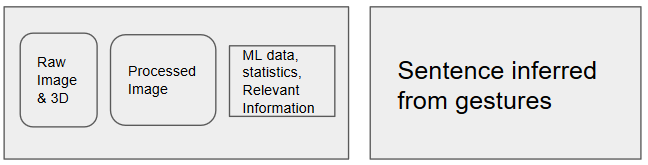
\includegraphics[width=150mm]{the_diagram_from_the_clients.png}
}
\vskip 0.2in
This layout will display to the user all relevant information that is calculated from our project. Beginning with the raw input they give to the camera, and ending with the final recognition made from our ML algorithm. This UI layout captures all parameters of our project, and will effectively allow a user to input gestures to the camera, and receive the ML classification.

\subsubsection{Design Concerns}
A few elements of the UI that could potentially go wrong are the connections between the camera and the UI and the connection between the ML and the UI.
Both of those connections are made through the SW team, which is imperative to the success of our project as a whole.
Any incorrect connections between the camera and the UI or the ML and the UI would result in loss of data or data misrepresentation. 
\subsubsection{Relationship}
The UI is one of the three parts of the application: the UI, the SW, and the ML. The UI is what the user will see and how the user will interact with   our project. Bridging the UI, the ML algorithm, and the camera is the SW project portions. The SW acts as a data exchange point between the UI and ML project portion. Lastly, the ML classifies the user input data (images) and uses the SW as a transfer pipeline to the UI to present the classification. Each individual component relies on the other to relay information through the project pipeline, resulting in a cohesive and interactive project. Below is a basic workflow pipeline of the interaction between the main project components:

\vskip 0.2in

\centerline{
   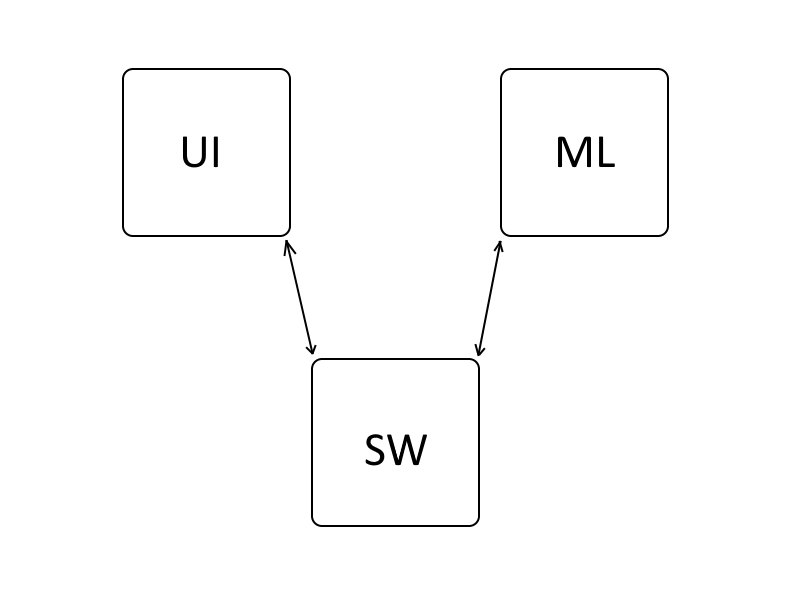
\includegraphics[width=65mm]{UI_graphic2.png}
}
\vskip 0.2in

\subsection{Viewpoint : Software Connectivity}
\subsubsection{Introduction}
This dependency aims to outline the interconnection between components that the SW project components should bring to our project.
Figure 2 below outlines the connection points that the software needs to create.
\begin{figure}[ht]
    \centering
    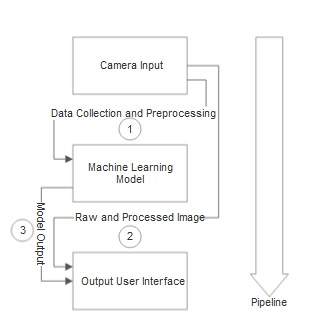
\includegraphics{SWDependency.png}
    \caption{Block Diagram Displaying Inter-connectivity of Software}
    \label{fig:Figure 4}
\end{figure}\\
The software aims to ease the sharing of data between different components of the project, and connect the input user interface to the machine learning model and output user interface.
\subsubsection{Data Collection and Preprocessing}
During data collection, the user interface will have a button to start capturing information.
This data needs to be preprocessed for the machine learning model.
The preprocessing design will start by extracting the depth per pixel image from the Intel RealSense Camera pipeline through the Intel RealSense SDK \cite{first}.
For training the machine learning model, the data will be added to a current HDF5 dataset after being normalized, and then saved for later training of the machine learning model.
For the real time testing and implementation of the machine learning model, this information will be directly sent after being normalized to the machine learning model, where it will be classified.
An example of normalization would go as follows: \\
\\$
\begin{bmatrix}
    0 & 0 & 0 & 0 \\
    1 & 1 & 2 & 1 \\
    1 & 2 & 3 & 4 \\
    1 & 1 & 0 & 1 \\
\end{bmatrix}
\xrightarrow{}
\begin{bmatrix}
    0 & 0 & 0 & 0 \\
    \frac{1}{4} & \frac{1}{4} & \frac{1}{2} & \frac{1}{4} \\
    \frac{1}{4} & \frac{1}{2} & \frac{3}{4} & 1 \\
    \frac{1}{4} & \frac{1}{4} & 0 & \frac{1}{4} \\
\end{bmatrix}
$ \\
\\
This technique will help our machine learning model be able to more easily recognize the same feature repeatedly, as all gestures will be scaled over the same interval $\mathbb{R} \rightarrow{} [0, 1]$.
\subsubsection{Raw and Processed Image}
The Raw and processed images need to be sent to the Output User Interface through a pipeline.
This can be done by building a function that can retrieve the current camera information from within the Output UI.
We will want two images to display within the user interface, the raw image, and the depth pixel image, that way the user can see what their gesture will be represented as.
There will be a separate function for retrieving the raw image and depth image.
\subsubsection{Model Output}
The model output needs to appear in the UI.
Once the data is put into the machine learning model, the data will be classified as a string and this result is what needs to appear on the user interface. It is imperative that connecting SW portions are ready to properly receive expected ML algorithm output format, and properly parse this for presentation to user via the UI.
\subsubsection{Design Concerns}
The main concerns for this section of the project is not over-promising on functionality. Not all of the team members are extremely familiar with  processing the images and normalization of data. The main problem would be able to get this section completed quickly enough, so that we can properly train the machine learning model with real data that has been normalized.

\subsubsection{Relationship}
This software section is hand-in-hand with the ML project portions. This needs to be done in order to build the database of training data that has been properly normalized. Furthermore, the UI team needs the initial GUI built so that we can have a housing application our group can use to actually begin the data collection process using the RealSense Cameras. 

\subsection{Viewpoint : Continuous Data Input}
\subsubsection{Introduction}
This information section will show how the software will deal with persistent data received from the camera. Specifically how the process will be able to take the camera input and classify the gesture real-time using the information that had been previously collected to train it. The gestures that it will be processing are ones that we are assuming the model has been previously trained for.

\subsubsection{Data Storage}
Before this project can classify real-time, it needs to be trained to recognize them.  After that, it will need a way to store the data it has collected to recognize performed gestures real-time. The original plan was to have a database connected to this project but at this point, the goal is just having accessible data without the hassle of retrieving it from a database. We will utilize an HDF5 file format that we can simply read for the model and will contain all of the input data. This will allow us to not waste time getting a database set up with the proper amount of data needed for ML model training.

\subsubsection{Design Concerns}
There are a few concerns for the data storage, namely that our group needs to ensure that the location where we store the HDF5 files is accessible for the machine learning model. Furthermore, there needs to be substantial space available on the drive for the files to be added and read from. Any issues with storage must be fleshed out as it can block our progress with the project overall, and impede our overall timeline.

\subsubsection{Relationship}
This section again is directly related to the ML team. The data we record must persist since the model will not be able to have accurate training without it. The data should be recorded via the first GUI interaction with the camera. It is imperative that the GUI application is ready to begin receiving camera input in order to begin implementation for this SW viewpoint.

\subsection{Viewpoint: Machine Learning Dependencies}
\subsubsection{Introduction}
The dependencies required by our Machine Learning model include the utilization of the Intel RealSense camera for model input, specified by our client, and the utilization of the PyTorch Deep Learning Framework to build the ML model. The camera input will ultimately feed the model, which will be created using PyTorch.
\subsubsection{Intel RealSense Camera Input}
The camera we will be using for our project is the Intel RealSense Depth Camera SR305. This indoor camera has an incredible quality of depth capturing capabilities, specifically when used under ideal conditions. Our group will utilize the existing Software Development Kit offered by Intel to utilize the camera's components to capture data. Specifically, in the context of our project's pipeline, the ML algorithm will receive camera input delivered from the UI portion of our project and processed by the SW pre-processing manipulations. Once the camera data reaches the ML algorithm, it will be ready for direct input into the model in order to yield a classification output. 
\subsubsection{PyTorch Deep Learning Framework}
Our group has chosen to implement a Deep Learning Convolutional Neural Network in order to accomplish the task of gesture recognition. Our group will be using the PyTorch Machine Learning Library Framework in order to begin building our Machine Learning Model. The PyTorch framework is geared to be more user-friendly than other frameworks in existence, and because the rest of our project is being built in Python it will allow for easier overall integration to utilize the PyTorch library built on top of the Python programming language. With this framework, our group will aim to build a Convolutional Neural Network algorithm to tackle the task of gesture recognition.
\subsubsection{Design Concerns}
The main concerns surrounding our group for both of these dependencies in the ML domain of our project involve the fact that this our group's first exposure to both of these tools. We will have to perform thorough research and development into both of these tools and their interactions, in order to be able to fully utilize these components for the ML project portions.
\subsubsection{Relationship}
The relationship involvement with the RealSense Camera dependency comes from both the UI viewpoint and the Software Connectivity viewpoint. User will need to interact with the UI in order to give input to the ML model, and the raw data will need to be manipulated prior to being fed to the model.
\subsection{Viewpoint: ML Algorithm}
\subsubsection{Introduction}
The chosen algorithm for our Machine Learning model is a Convolutional Neural Network (CNN). This algorithm will be the driving force behind our project's capability of recognizing human hand gestures. The algorithm will be built by using the PyTorch Deep Learning Framework, and will make the ultimate gesture recognition predicition for our project.
\subsubsection{Convolutional Neural Network}
The nature of our project ultimately boils down to a computer vision problem, where our group is tasked with creating a computer program capable of recognizing human hand gestures coming from the Intel RealSense Camera. While there are many ways our group may choose to approach the implementation for this task, our group went with likely the most promising avenue at our disposal, which is a Machine Learning algorithm. Within the domain of Machine Learning, there exists multiple different types of algorithms each with their own strengths and weaknesses. As of recent, one particular ML algorithm known as Convolutional Neural Networks has shown astounding capabilities in it's ability to perform ML tasks\cite{first}. For this reason, this is the ML algorithm that our group has chosen to implement for our gesture recognition task. 
\\
\begin{figure}[ht]
    \centering
    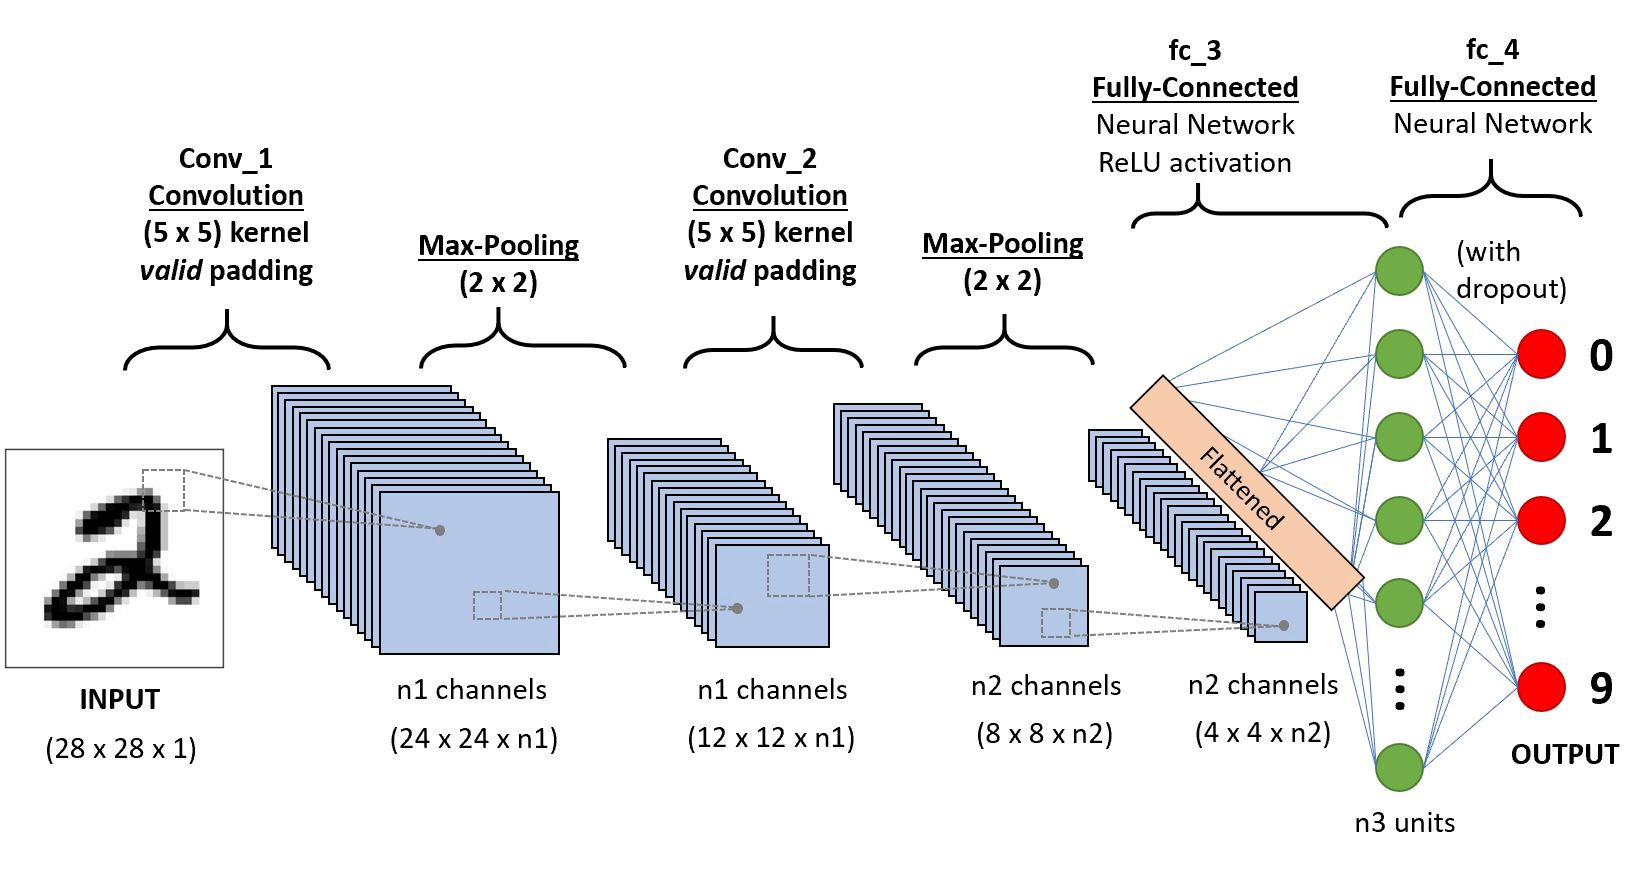
\includegraphics[width=.8\textwidth]{CNN.jpeg}
    \caption{CNN Architecture Diagram\cite{first}}
    \label{fig:Figure 5}
\end{figure}
\\
 A pictorial representation of the Convolutional Neural Network pipeline can be seen above, with a single image input example. A high level look at this algorithm reveals a sophisticated computational graph that is comprised of several layers working together to accomplish a machine learning task. A deeper dive into the algorithm reveals three major layer types that compose the CNN architecture; the Convolutional Layer, the Pooling Layer, and the Fully Connected Layer. These three layers are sequentially connected and result in sophisticated computation graphs that performs very well in machine learning tasks. The Convolutional layer performs image dimension reduction, and extract the high level features of the input image such as edges and colors. The Pooling layer takes the output from the convolutional layer and performs spatial reduction on the newly represented dataset. In this process dominant features are extracted and noisy features are ignored which results in higher accuracy models. Lastly, the Fully Connected layer takes the pooling layer output and performs calculations to make the algorithm’s ultimate prediction\cite{first}.


\subsubsection{Design Concerns}
One of the main design concerns involved with this chosen algorithm is simply the complexity of such an implementation. The area of machine learning is an active area of research, and specifically CNN research due to its recent success. This being said, our group will likely have a steep learning curve with this chosen implementation. Furthermore, this algorithm requires a large training set to properly learn its given task. Our group will have to build this training database from scratch, and this leads to concerns of time constraints. Our group will not only have to properly build this algorithm, but also create the training sets needed for a thorough implementation.
\subsubsection{Relationship}
This viewpoint directly relations with the Machine Learning dependency viewpoint, as the PyTorch framwork will be used to build this algorithm. Furthermore, the Machine Learning Connectivity Viewpoint is a direct relationship to this algorithm, as each connection that is highlighted through that viewpoint will have direct interaction with the algorithm highlighted in this viewpoint. These two interactions are vital for the smooth implementation of this design viewpoint.
\subsection{Viewpoint: Machine Learning Connectivity}
\subsubsection{Introduction}
The ML portion of our project must interact with the two other major components of our project, being the UI and SW portions. Our project will initially require a user to interact with the UI to provide input data to SW project portions, which will perform pre-processing manipulations to provide direct input the ML algorithm. The ML algorithm will then provide it's gesture classification output back to the SW portion which will parse the information, and ultimately present the classification in the UI to the user. 
\subsubsection{UI Interaction}
The UI interactions with the ML project portions are indirect, with the SW portion mediating the data exchange between the two. Although the relationship is indirect, it is dire that the information exchange between the two is accurate, as they are the raw truths as to what the direct camera inputs and direct classification outputs are. It is important to establish a firm pipeline connection between these entities in order to ensure the creation of best possible application we can feasibly produce. The main way this can be accomplished is through a solid mediator, being the SW portion of our project.
\subsubsection{SW Interaction}
The SW interactions with the ML project components are direct, with the output from the SW portion directly feeding the ML algorithm, and the ML algorithm's output directly being fed back to SW portions for parsing and presentation. The interactions between these two components are essential to our project's success, and we must ensure that the correct pre-processing occurs to the data, in the context of our selected ML algorithm. Furthermore, we must ensure that the SW is ready to receive expected ML output formats so that it may correctly parse this information, perform any required performance metrics, and securely present this information to the user via the UI. These connection components must be thoroughly tested to ensure the quality of our project's information retrieval and presentation.
\subsubsection{Design Concerns}
The design concerns for this viewpoint mainly arise for the direct interactions taken between the ML and SW project portions. Because the SW project portion will act as a data exchange between the UI and ML algorithm, it is imperative that a proper data hand-off occurs between these components. The pre-processing manipulations (explained in the Software Connectivity Viewpoint) must be properly formed for input to the ML algorithm, and these same SW portions must be ready to handle the output format of the ML algorithm. These connections must be thoroughly tested to ensure project integrity.
\subsubsection{Relationship}
One main relationship for this viewpoint is the ML algorithm viewpoint. The main reason for this relationship is again, the fact that a proper data exchange must occur between SW and ML project portions in order to ensure the accuracy of information displayed to the user. Furthermore, this relationship cascades to the UI viewpoint, as the user will ultimately input directly to ML portions, and see the output of ML calculations.

\subsection{Viewpoint: Machine Learning Required Resources}
\subsubsection{Introduction}
The process by which our group will train and test the validation of our ML algorithm's gesture recognition capabilities is through a collection of training sets created by our group, using the Intel RealSense cameras. Our group will utilize on-campus computing resources to tackle the large computational cost required to thoroughly process these training sets through our algorithm.
\subsubsection{Machine Learning Training Data}
The training data we will use to train our ML algorithm for the gesture recognition task will be the most vital data aspect of our project. There is a high importance in obtaining plentiful and quality forms of training data, portraying a wide range of possible motions for a single given gesture. Our group has established base guidelines when capturing data, such as requiring that gestures be captured under the ideal condition of a one meter distance from the camera. Quantitative measures such a total number of videos per gesture, and video length per gesture will be determined immediately upon foundational building of our ML algorithm.
\subsubsection{Computational Resources}
The computational cost required by our project to sufficiently train the ML model for gesture recognition is going to be more than just a single group member’s machine can handle. The complexity of the algorithms used to build ML models will require high computational power, and therefore require our group to utilize methods for multiplying computational powers. Our group's chosen option for this need is to utilize the in-house computing cluster hosted on OSU's server. This parallelized computing resource will help mitigate wait times caused by complex computations, and be a highly beneficial component to the ML portion of our project. Although this will mainly affect the training/testing phases, it will help ensure a higher quality ML algorithm as a result. 
\subsubsection{Design Concerns}
The design concerns associated with this viewpoint mainly revolve around the required machine learning data for this project. The concern is the amount of data that is required to properly train the algorithm for the recognition task at hand, and the fact that our group must build this training set from scratch. The main concern ultimately boils down to a worry of lack of time for the sheer amount of work involved in this project. Our group will aim to follow the timeline described above, and hope that this is enough to time implement all portions of our project.
\subsubsection{Relationship}
The relationship this viewpoint holds to other viewpoints is mainly concerned with the Software Connectivity viewpoint, and specifically the data collection domain. The form of data collection outlined in the Software Connectivity viewpoint will dictate the data form that collected training sets will take. This will also dictate the form of input taken by the ML algorithm, and will help guide the building of this algorithm. 
\section{Design Rationale}
\subsection{Pipeline}
 The project structure is a sequential pipeline. The goal of this structure is to be able to divide the project into parts that can be developed, tested, and function on their own with simulated inputs and outputs. Eventually each part of the pipeline will be connected to create the complete product. The following figure explains the connections within the pipeline.\\
 \begin{figure}[ht]
    \centering
    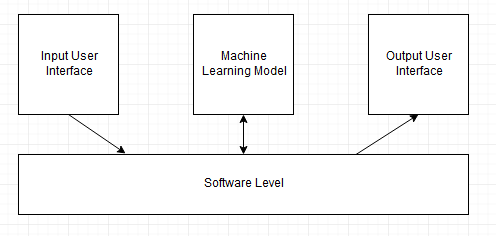
\includegraphics[width=.8\textwidth]{pipeline.png}
    \caption{Pipeline and Connectivity Diagram}
    \label{fig:Figure 6}
\end{figure}\\
The rationale behind this structure is the Dependency Inversion Principle. We would like all of the parts to be simulated and function on their own, but once all of the modules are built, they need to depend on each other. This design helps us be able to build our product in parallel so that there is more time for bug fixing, testing, and training of our machine learning model. The project is data driven, and thousands of image data needs to be captured and stored into our data storage method. This design allows us to develop certain parts of the project while gathering our data set, which will be time consuming and done manually. This pipeline model outlines the interactions for our project's separate components.

\newpage
\begin{thebibliography}{9}

\bibitem{first} 
Saha, S. 
\textit{A Comprehensive Guide to Convolutional Neural Networks — the ELI5 way}. 
Towards Data Science, 2018. Retrieved on November 10, 2019 from https://towardsdatascience.com/a-comprehensive-guide-to-convolutional-neural-networks-the-eli5-way-3bd2b1164a53.

\end{thebibliography}
\end{document}